\documentclass[12pt,twoside,book]{article}
\usepackage{docmute}

\input{../settings}

\begin{document}

%%%%%%%%%%%%%%%%%%%%%%%%%%%%%%%%%%%%%%%%%%%%%%%%%%%%%%%%%%%%%%%%%%%%%%%%%%%%%%%
\section{Models with WIMPs}
\setcounter{equation}{0}
%%%%%%%%%%%%%%%%%%%%%%%%%%%%%%%%%%%%%%%%%%%%%%%%%%%%%%%%%%%%%%%%%%%%%%%%%%%%%%%

\vskip 0.1in

There are several examples of the models that contain WIMP DM
candidates.  In this section, two of them \rem{Really?} are briefly
reviewed.  \rem{EWIMP and WIMP??}

%%%%%%%%%%%%%%%%%%%%%%%%%%%%%%%%%%%%%%%%%%%%%%%%%%%%%%%%%%%%%%%%%%%%%%%%%%%%%%%
\subsection{Minimally supersymmetric standard model}
%%%%%%%%%%%%%%%%%%%%%%%%%%%%%%%%%%%%%%%%%%%%%%%%%%%%%%%%%%%%%%%%%%%%%%%%%%%%%%%

The minimally supersymmetric standard model (MSSM) is the simple extension of the SM with $\mathcal{N} = 1$ supersymmetry (SUSY).
For a brief review of the $\mathcal{N} = 1$ SUSY, see Sec.~\ref{sec:susy}.
SUSY is well-motivated since it provides a good solution to the so-called hierarchy problem.~\cite{Weinberg:1975gm,Gildener:1976ai,Susskind:1978ms}.


\begin{figure}[b]
  \centering
  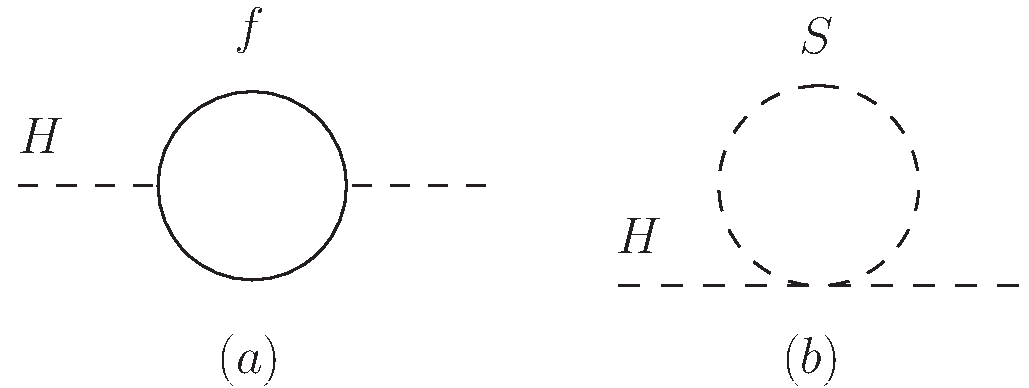
\includegraphics[width=0.6\hsize]{Higgs_mass.pdf}
  \caption{One-loop correction to the Higgs mass from (a) a fermion $f$ and (b) a scalar $S$.}
  \label{fig:Higgs_mass}
\end{figure}

We summarize the notations and quantum numbers of the chiral and vector superfields in the MSSM in Table~\ref{tab:mssm_csf} and \ref{tab:mssm_vsf}, respectively.
The supersymmetric part of the MSSM lagrangian is described by the superpotential
\begin{align}
  W = Y_u^{i j} U_i Q_j H_u - Y_d^{i j} D_i Q_j H_d
  - Y_e^{i j} E_i L_j H_d + \mu H_u H_d,
  \label{eq:mssm_sup}
\end{align}
where $i,j=1,2,3$ labels the quark and lepton generation, while $Q, L, U, D, E$ are superfields that contain the left-handed quark, left-handed lepton, right-handed up-type quark, right-handed down-type quark, and right-handed charged lepton, respectively.
In Eq.~\eqref{eq:mssm_sup}, proper contraction of $SU(3)_C$ and $SU(2)_L$ indices is assumed.
Note that two Higgs doublets $H_u$ and $H_d$ with opposite values of $U(1)_Y$ hypercharges are introduced, which is needed to cancel the contributions to the gauge anomaly from Higgs superpartners, Higgsinos.

Since no superpartner of any SM particle is observed yet, SUSY should be broken and superpartners should obtain the SUSY breaking masses.  \rem{ref: boson and fermion obtain equal mass}
The SUSY breaking part of the lagrangian is expressed as
\begin{align}
  \mathcal{L}_{\mathrm{soft}} =&
  -\frac{1}{2} \left( M_3 \g \g + M_2 \W \W + M_1 \B \B + \mathrm{c.c.} \right) \notag \\&
  -\left( A_u^{ij} \U_i \Q_j H_u - A_d^{ij} \D_i \Q_j H_d - A_e^{ij} \E_i \L_j H_d \right) \notag \\&
  -m_Q^{2ij} \Q^\dagger_i \Q_j - m_L^{2ij} \L^\dagger_i \L_j - m_U^{2ij} \U^\dagger_i \U_j
  -m_D^{2ij} \D^\dagger_i \D_j - m_E^{2ij} \E^\dagger_i \E_j \notag \\&
  -m_{H_u}^2 H_u^{*} H_u - m_{H_d}^2 H_d^{*} H_d - \left( b H_u H_d + \mathrm{c.c.} \right),
  \label{eq:mssm_soft}
\end{align}
where the tilde is used to express the superpartner of the SM particle contained in a superfield, while a field without a hat nor tilde denotes the other component.



\begin{table}[t]
  \centering
  \begin{tabular}{c|ccc}
    Notation & $SU(3)_C$ & $SU(2)_L$ & $U(1)_Y$ \\ \hline
    $\hat{Q}_i$ & $\bm{3}$ & $\bm{2}$ & $1/6$ \\
    $\hat{L}_i$ & $\bm{1}$ & $\bm{2}$ & $-1/2$ \\
    $\hat{U}_i$ & $\bar{\bm{3}}$ & $\bm{1}$ & $-2/3$ \\
    $\hat{D}_i$ & $\bar{\bm{3}}$ & $\bm{1}$ & $1/3$ \\
    $\hat{E}_i$ & $\bm{1}$ & $\bm{1}$ & $1$ \\
    $\hat{H}_u$ & $\bm{1}$ & $\bm{2}$ & $1/2$ \\
    $\hat{H}_d$ & $\bm{1}$ & $\bm{2}$ & $-1/2$
  \end{tabular}
  \caption{Notations and quantum numbers of the chiral superfields in the MSSM.}
  \label{tab:mssm_csf}
\end{table}

\begin{table}[t]
  \centering
  \begin{tabular}{c|ccc}
    Notation & $SU(3)_C$ & $SU(2)_L$ & $U(1)_Y$ \\ \hline
    $\hat{g}$ & $\bm{8}$ & $\bm{1}$ & $0$ \\
    $\hat{W}$ & $\bm{1}$ & $\bm{3}$ & $0$ \\
    $\hat{B}$ & $\bm{1}$ & $\bm{1}$ & $0$ \\
  \end{tabular}
  \caption{Notations and quantum numbers of the vector superfields in the MSSM.}
  \label{tab:mssm_vsf}
\end{table}



\begin{table}
 \centering
 \begin{tabular}{c|ccc|cc}
  & \multicolumn{3}{c|}{Quntum numbers} & \multicolumn{2}{c}{Masses}\\
  WIMP DM candidate & $SU(2)_L$ & $U(1)_Y$ & Spin & $m_\chi / \mathrm{TeV}$ &
  $\Delta m_\chi / \mathrm{MeV}$ \\
  \hline
  Higgsino & $2$ & $1/2$ & Dirac fermion & 1.1 & 341 \\
  Wino & $3$ & $0$ & Majorana fermion & 2.9 & 166 \\
  5-plet scalar & $5$ & $0$ & real scalar & 9.4 & 166 \\
  5-plet fermion & $5$ & $0$ & Majorana fermion & 10 & 166
 \end{tabular}
 \caption{Table of properties of popular WIMP DM
 candidates~\cite{Farina:2013mla, ArkaniHamed:2006mb, Hisano:2006nn,
 Cirelli:2007xd, Moroi:2013sla, Beneke:2016ync}.  The $SU(2)_L$
 electroweak charge, $U(1)_Y$ hypercharge, spin nature, mass, and mass
 difference compared with a charged component of the multiplet are
 shown.  See Sec.~\ref{???}  \rem{Caution!!} for the details of the last
 column.}  \label{tab_WIMP_property}
\end{table}


\rem{Relationship between $\lambda$ parameter above should be clearer}
WIMPs with mass around or just above the electroweak scale are
theoretically well-motivated in connection with problems of the SM such
as the naturalness problem.  For example, the minimal supersymmetric
extension of the SM (the so-called MSSM) contains several WIMP DM
candidate such as Higgsino and Wino.\footnote{
%%
For a review of the MSSM, see for example~\cite{Martin:1997ns}.
}
%%
Another example is the minimal dark matter (MDM)
model~\cite{Cirelli:2005uq, Cirelli:2007xd, Cirelli:2009uv}, which is a
simple extension of the SM with an $SU(2)_L$ electroweak multiplet such
as a $5$-plet scalar / fermion.  In these models, the stability of the
DM is ensured by the $R$-parity (for the MSSM case) and by high
dimensionality of the operator that describes the decay of the DM (for
the MDM case).  The properties of these WIMP DM candidates are
summarized in Table~\ref{tab_WIMP_property}.  The required masses to
explain the DM relic abundance through the freezeout mechanism are also
shown.  Since the non-relativistic annihilation cross section of
$\mathrm{TeV}$ mass particles is significantly enhanced by the
Sommerfeld enhancement effect~\cite{Hisano:2004ds, Hisano:2006nn}, there
are deviations from the rough estimation formula
Eq.~\eqref{eq_relic_abundance}.  We will return to this point later in
Sec.~\ref{???}.  \rem{Caution!!}  In addition, in the last column there
are mass differences $\Delta m_\chi$ between the DM and its charged
couterpart that will be explained in detail in Sec.~\ref{???}.
\rem{Caution!!}

%%%%%%%%%%%%%%%%%%%%%%%%%%%%%%%%%%%%%%%%%%%%%%%%%%%%%%%%%%%%%%%%%%%%%%%%%%%%%%%
\subsection{Minimal dark matter model}
%%%%%%%%%%%%%%%%%%%%%%%%%%%%%%%%%%%%%%%%%%%%%%%%%%%%%%%%%%%%%%%%%%%%%%%%%%%%%%%



\bibliographystyle{elsarticle-num}
\bibliography{../phd}

\end{document}
